\chapter{Menjalankan \textbf{\textit{Python}}}

\section{Menjalankan script python dengan perintah CLI}
Untuk menjalankan perintah CLI cukup mudah yaitu sebagai berikut

\begin{enumerate}

\item Buka terminal lalu ketikkan \textbf{python \textit{namafile}.py} seperti gambar ~\ref{cli}, lalu enter
\begin{figure}[H]
\centering
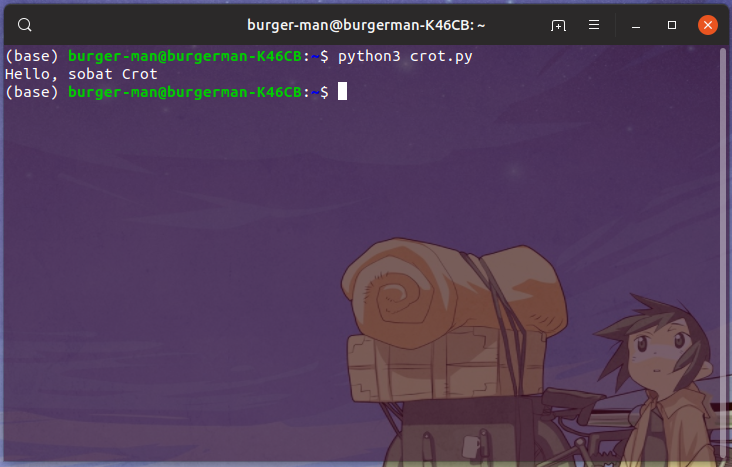
\includegraphics[width=1\textwidth]{figures/cli.png}
\caption{Gambar running script dengan CLI}
\label{cli}
\end{figure}

\end{enumerate}

\section{Hello World!}
Sekarang kita akan menjalankna perintah Hello World! pada IDE spyder caranya sebagai berikut
\begin{enumerate}
\item Buka IDE spyder
\item Lalu kita ketikkan perintah seperti gambar \ref{helloworld}, lalu kita run dengan memencet tombol \textbf{F5} atau dengan mengklik tombol play di bagian toolbar IDE
\begin{figure}[H]
\centering
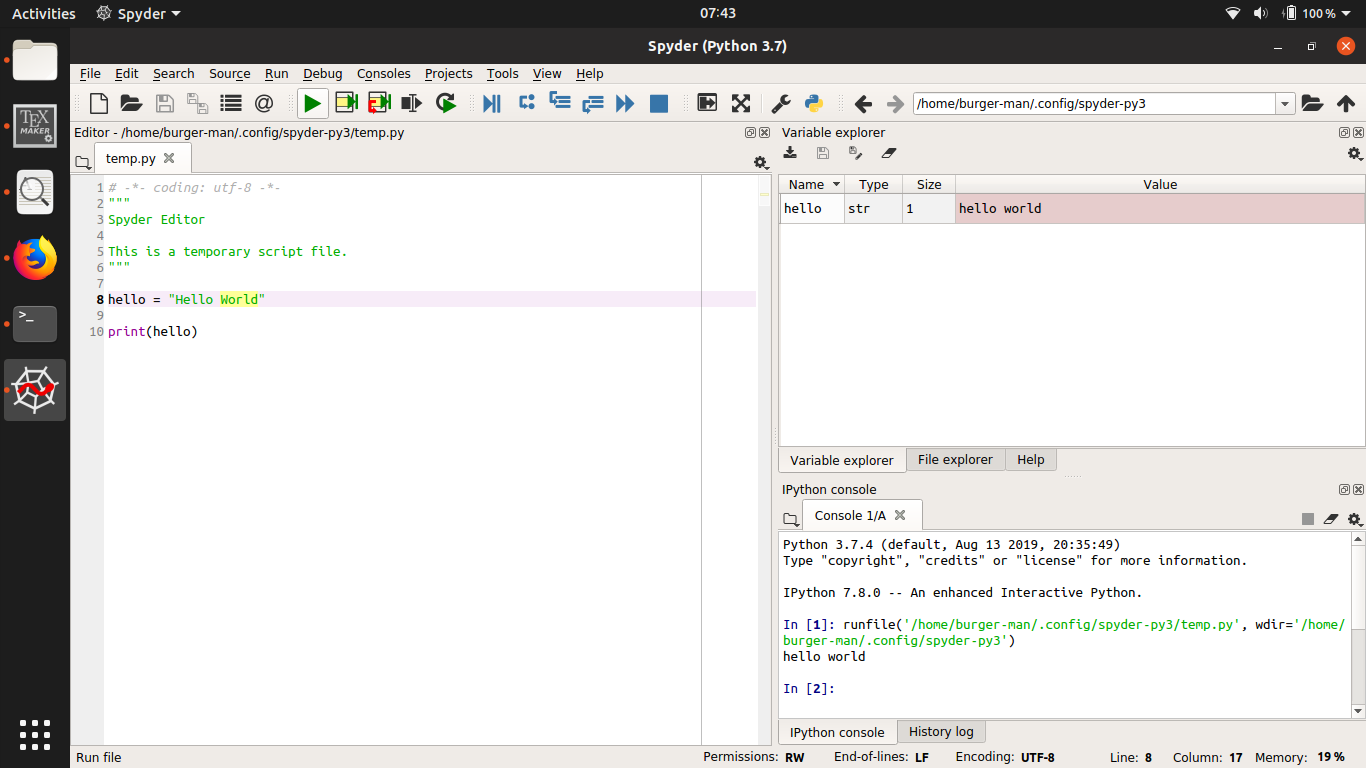
\includegraphics[width=1\textwidth]{figures/helloworld.png}
\caption{Gambar running script dengan spyder}
\label{helloworld}
\end{figure}
\end{enumerate}

\section{Auto Login SIAP}
Now, kita akan mencoba menjalankan script python auto login ke halaman siap.poltekpos.ac.id, let'ssss goooo

\begin{enumerate}
\item kunjungi laman \textbf{\textit{https://github.com/trianggadios/autologinsiap}} seperti gambar \ref{webgithub}
\begin{figure}[H]
\centering
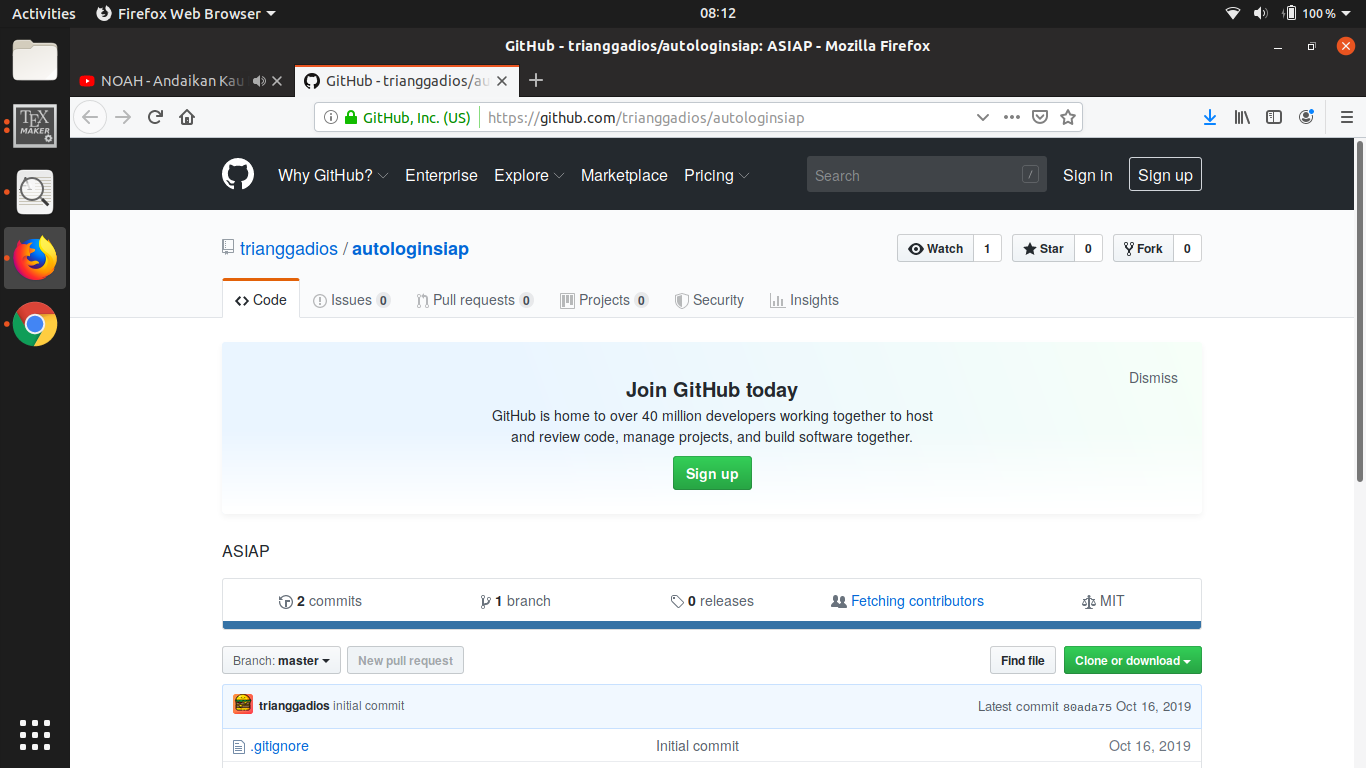
\includegraphics[width=1\textwidth]{figures/webgithub.png}
\caption{Gambar halaman github}
\label{webgithub}
\end{figure}

\item clone atau download repo tersebut
\item masuk ke direktori repo tersebut dan kita akan menemukan file \textbf{\textit{main.py}} kita klik kanan dan open dengan Spyder IDE seperti gambar \ref{openwithspyder}
\begin{figure}[H]
\centering
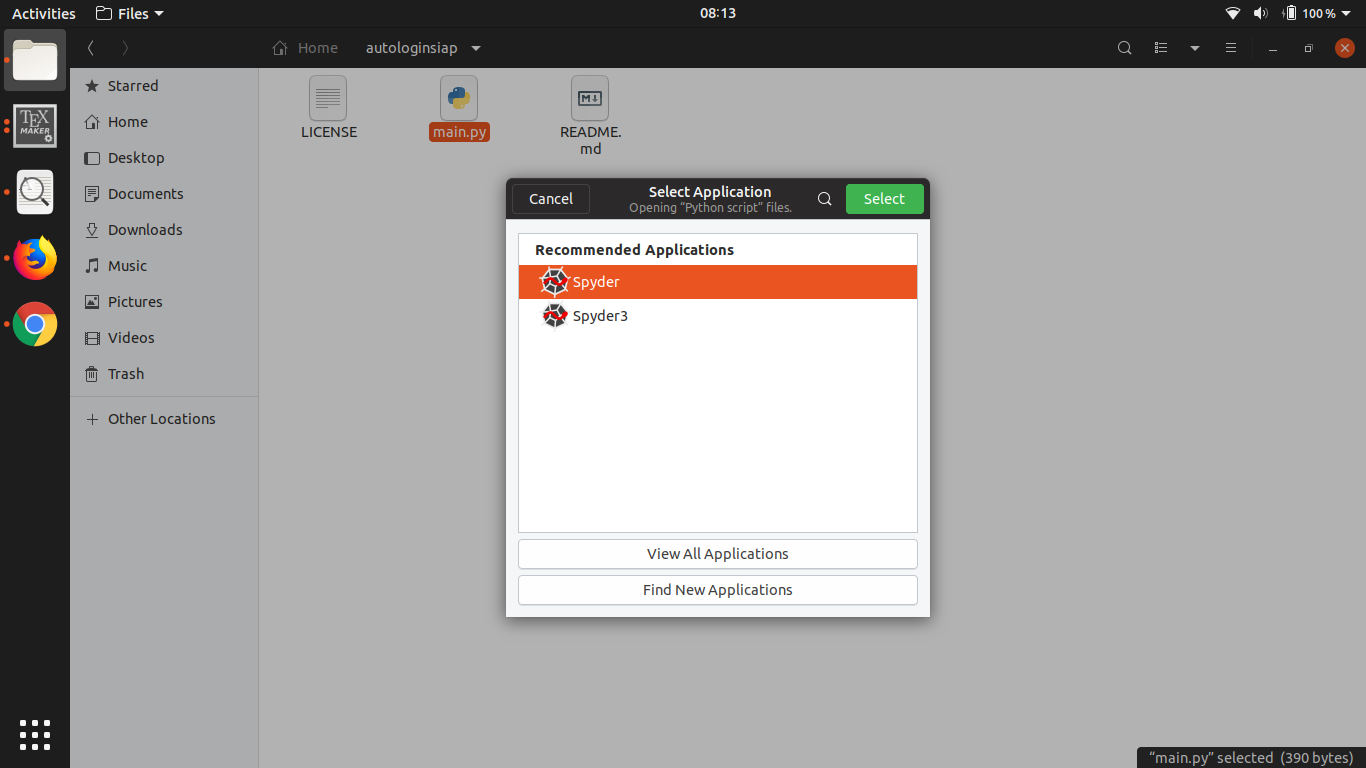
\includegraphics[width=1\textwidth]{figures/openwithspyder.png}
\caption{Gambar open dengan spyder}
\label{openwithspyder}
\end{figure}

\item setelah itu kita run file tersebut, dan masukkan npm dan password siap kita dengan benar

\end{enumerate}

\section{Menggunakan Variable Explorer}
Menggunakan Variable Explorer ini cukup simple yaitu fungsinya untuk mengetahui apa nama variabel tersebut, type datanya, jumlahnya, dan isinya apa. Berikut contohnya di gambar \ref{variabel}
\begin{figure}[H]
\centering
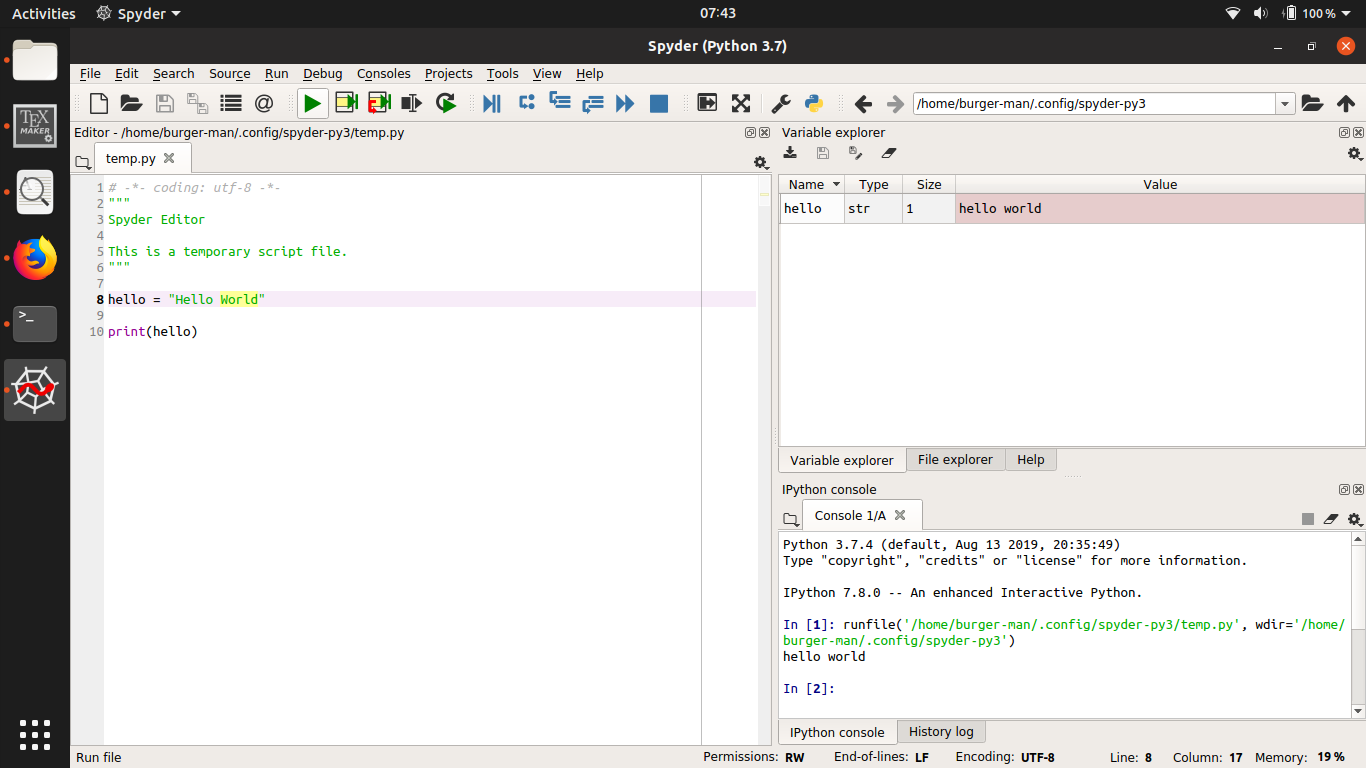
\includegraphics[width=1\textwidth]{figures/helloworld.png}
\caption{Gambar running script dengan spyder}
\label{variabel}
\end{figure}

Dikanan atas ada field yang menyebutkan variable explorer dan disitu terlihat bahwa di program yang kita tulis seperti tabel \ref{vexplorer}
\begin{table}[H]
\centering
\begin{tabular}{|l|l|}
\hline
name      & hello       \\ \hline
type data & str         \\ \hline
syze      & 1           \\ \hline
value     & hello world \\ \hline
\end{tabular}
\caption{Tabel variabel explorer}
\label{vexplorer}
\end{table}

\section{Identasi}
Apa itu indentasi? indentasi adalah sebuah aturan python dimana untuk menentukan pembuka dan penutup pada program python biasanya indentasi digunakan setelah sintaks yang menggunakan tanda \textbf{:}, contoh pada gambar \ref{indentasi}
\begin{figure}[H]
\centering
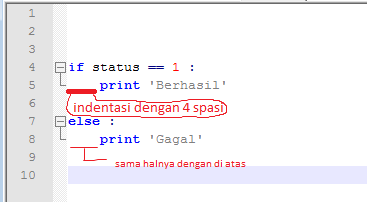
\includegraphics[width=1\textwidth]{figures/indentasi.png}
\caption{Gambar contoh indentasi}
\label{indentasi}
\end{figure}

Jika indentasi ada yang salah maka akan seperti gambar \ref{errorindentasi}
\begin{figure}[H]
\centering
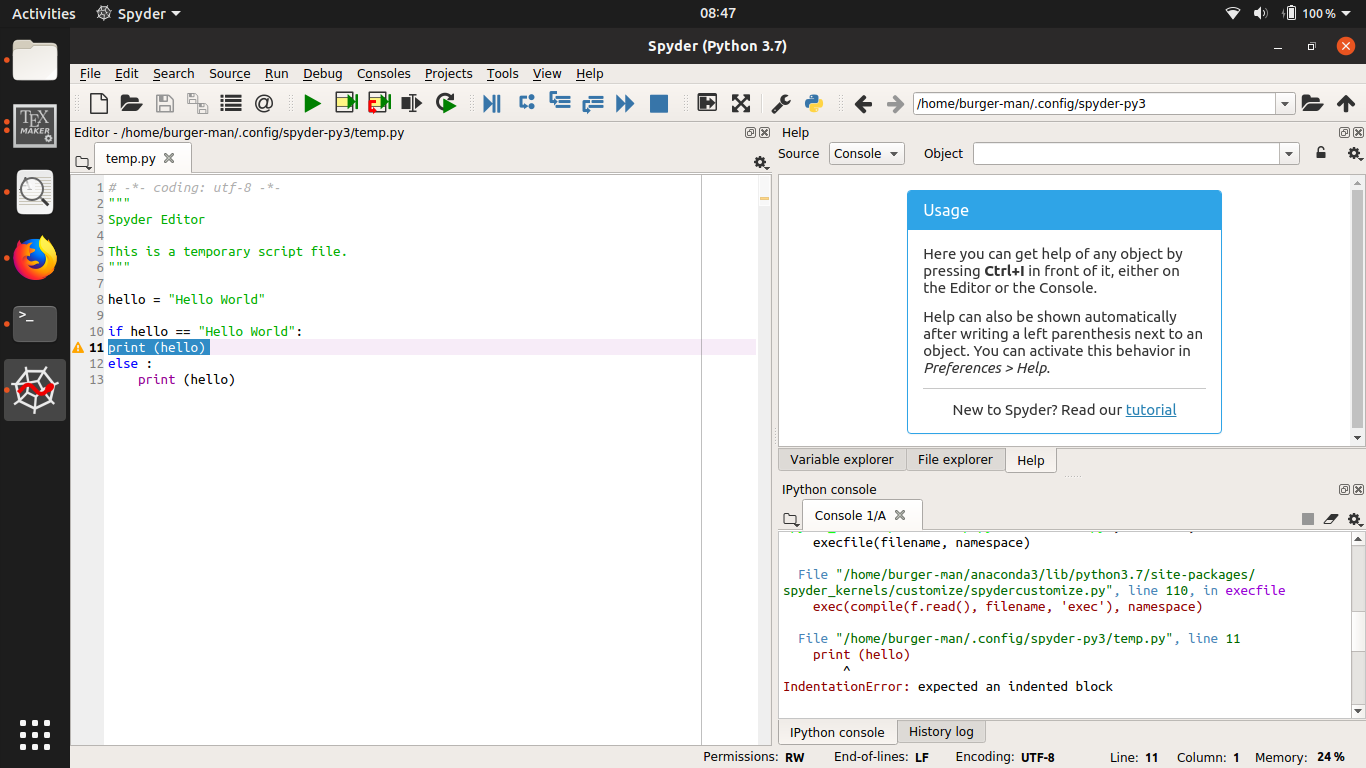
\includegraphics[width=1\textwidth]{figures/errorindentasi.png}
\caption{Gambar contoh error indentasi}
\label{errorindentasi}
\end{figure}

Gambar diatas jelas sekali salah karena setelah sintaks \textbf{if hello == "hello world" :} yang memiliki tanda \textbf{:} tidak menjorok sebesar 4 spasi

Cara membaca error tersebut adalah dengan membaca line berapa yang error? pada gambar \ref{errorindentasi} terlihat jelas bahwa yang error \textbf{\textit{line 11}} sehingga kita mengetahui line berapa yang error, selanjutnya kita baca apa yang error? disitu tertulis yang error adalah \textbf{\textit{expected and indented block}} yang artinya di line 11 indentasinya salah atau ada yang terblokir di proses itu.

sehingga penanganan errornya seperti berikut
\begin{enumerate}

\item Kita sejajarkan dahulu line yang bermasalah dengan line yang diatasnya seperti gambar \ref{benerin1}
\begin{figure}[H]
\centering
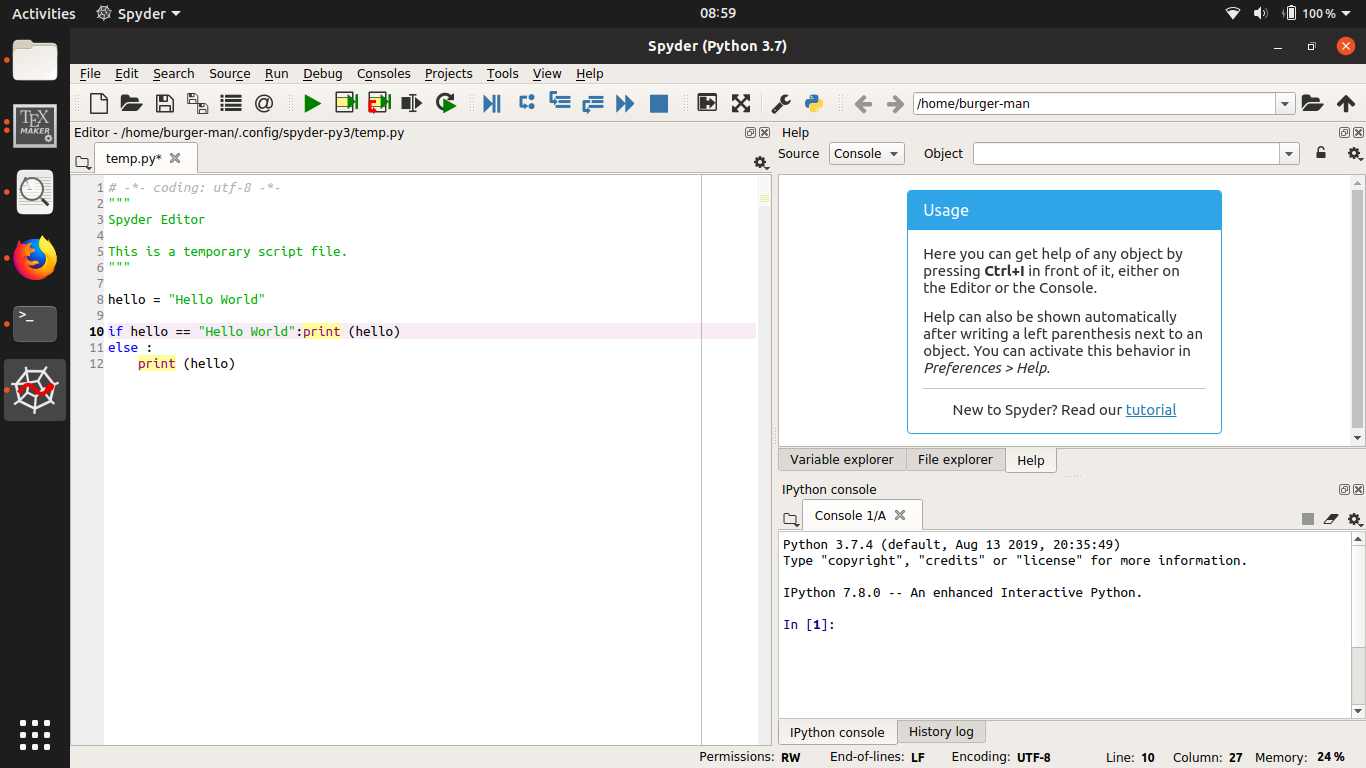
\includegraphics[width=1\textwidth]{figures/benerin1.png}
\caption{Gambar penanganan indentasi 1}
\label{benerin1}
\end{figure}

\item setelah itu kita tekan enter hingga menjadi benar seperti gambar \ref{benerin2}
\begin{figure}[H]
\centering
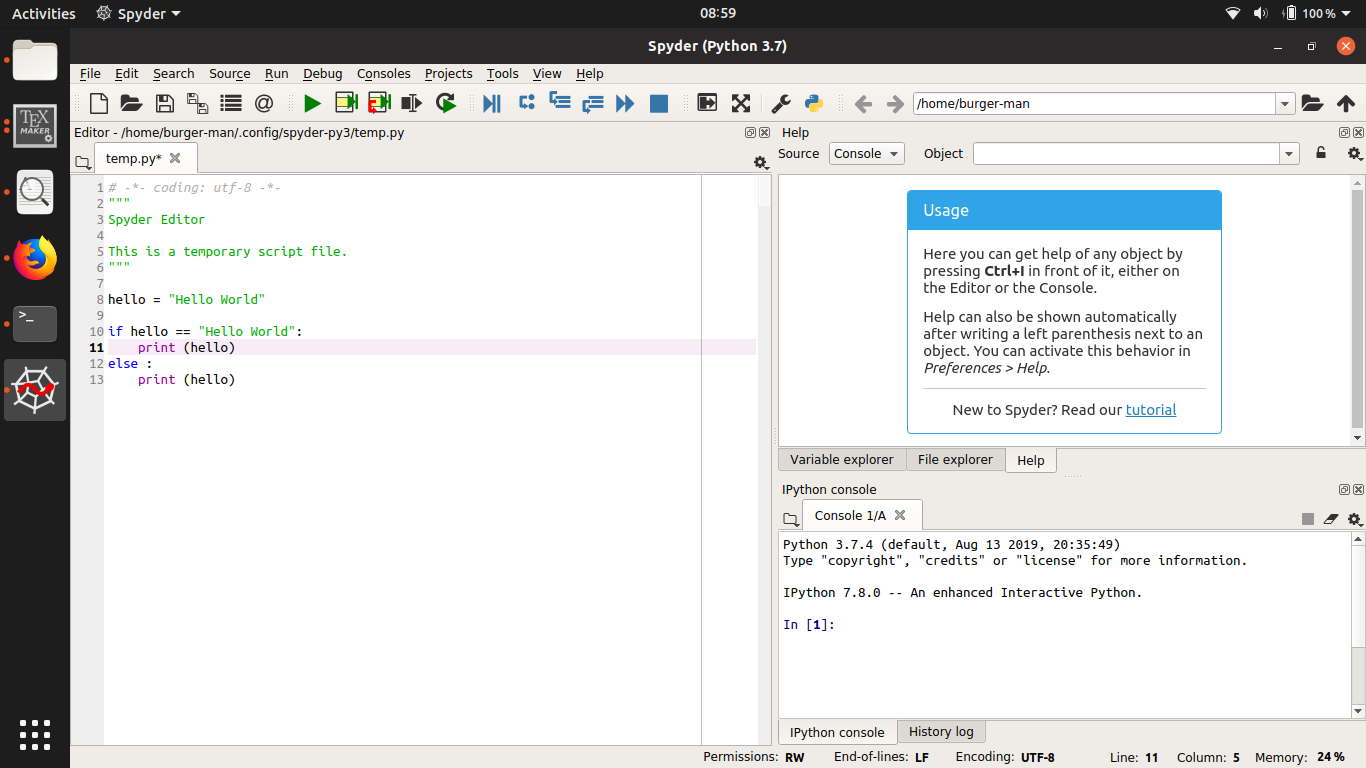
\includegraphics[width=1\textwidth]{figures/benerin2.png}
\caption{Gambar penanganan indentasi 2}
\label{benerin2}
\end{figure}

\end{enumerate}